\documentclass[11pt,a4paper]{article}

\usepackage[T1]{fontenc}
\usepackage{lmodern}
\usepackage[margin=2.5cm]{geometry}
\usepackage{graphicx}
\usepackage{booktabs}
\usepackage{float}
\usepackage{caption}
\usepackage{subcaption}
\usepackage[hidelinks]{hyperref}

% Figures and tables come from the training notebook; see docs/build_tables.py.
\graphicspath{{../notebooks/outputs/phase1/}}
\captionsetup{font=small,labelfont=bf}

% Replace with the names of the team members before submitting.
\newcommand{\reportauthors}{Team members}

\title{From Pixels to Predictions\\[0.3em]
\large Phase 1 report: training dataset construction and preliminary models}
\author{\reportauthors\\[0.3em] ML101 Final Project}
\date{November 13, 2026}

\begin{document}
\maketitle

\section{Scope}

This report covers the first phase of the project: how the tabular training
dataset was built from the Sentinel-2 scene and the ground-truth polygons, and
the preliminary evaluation of three of the six classification architectures.
For each model it reports the confusion matrix and the overall accuracy, as
required for this phase. Hyper-parameter optimisation, the remaining three
architectures and the full-scene inference belong to phase 2.

\section{Source data}

\paragraph{Scene.} A Sentinel-2 Level-2A product over Bogot\'a, tile T18NWL,
acquired on August 10, 2026. It provides ten spectral bands (B01, B02, B03,
B04, B05, B06, B07, B8A, B11 and B12) as JPEG~2000 files resampled to 20~m.
Every band is a $5490 \times 5490$ grid of 16-bit unsigned integers in the
coordinate reference system WGS~84 / UTM zone 18N (EPSG:32618).

\paragraph{Ground truth.} A table of 11,711 polygons, each one with its
geometry in well-known text, an identifier and the integer class label. The
file does not declare a coordinate reference system; its extent coincides
exactly with the extent of the tile in EPSG:32618, which is therefore the
system assumed. The labels follow the convention of the project brief, and
the polygons cover classes 2 to 10; classes 0, 1 and 11 are not present.

\section{Construction of the TSV training dataset}

\subsection{Pipeline}

The dataset is built by three Airflow workflows that move the data through
three layers, each one stored and never overwritten by the next:

\begin{enumerate}
  \item \textbf{Source files.} The ten bands are uploaded unchanged to an
  object store (MinIO), and the polygons are loaded as they come into the
  PostGIS table \texttt{raw.polygon\_classes}. The polygon file is validated before
  loading: expected columns, integer identifiers and labels, no empty
  geometry and no repeated identifier.
  \item \textbf{Extracted pixels.} Every pixel that belongs to a polygon is
  stored with its ten band values, its coordinates, its class and the
  identifier of its polygon (\texttt{extracted.polygon\_pixels}). Nothing is
  filtered at this stage.
  \item \textbf{Training samples.} The extracted pixels are cleaned and stored
  one row per pixel (\texttt{training.samples}), and exported as the TSV file.
\end{enumerate}

The extraction is written in Python with \texttt{rasterio} to read the bands
and \texttt{shapely} to handle the geometries; no GIS desktop software is
involved.

\subsection{Extraction rules}

\begin{itemize}
  \item \textbf{Pixel membership.} A pixel belongs to a polygon when the centre
  of the pixel lies inside the polygon. Each polygon is rasterised on its own
  window of the grid, so a pixel covered by two polygons is recorded once per
  polygon and the overlap can be examined later.
  \item \textbf{Band values.} The ten values of a pixel are the digital numbers
  stored in the band files, without rescaling. Before sampling, the workflow
  checks that the ten bands share the same grid (reference system, origin,
  resolution and size) and that this system is the one of the polygons.
  \item \textbf{Coordinates.} The centre of each pixel is transformed from
  EPSG:32618 to geographic coordinates (EPSG:4326) to obtain the latitude and
  the longitude required in the table.
  \item \textbf{Class label.} Each pixel takes the label of its polygon.
\end{itemize}

\subsection{Cleaning rules}

Three rules are applied when the training samples are built: a pixel is
dropped when any of its bands has no data (value 0); a pixel is dropped when
it is claimed by polygons of different classes, because its label is
ambiguous; and a pixel covered more than once by polygons of the same class is
kept once. In this dataset none of the rules removed anything: the 583,835
extracted pixels are 583,835 distinct pixels with data in every band and a
single class.

\subsection{Resulting table}

The TSV file has 583,835 rows and thirteen columns, in this order:
\texttt{Latitude}, \texttt{Longitude}, the ten bands (\texttt{B01},
\texttt{B02}, \texttt{B03}, \texttt{B04}, \texttt{B05}, \texttt{B06},
\texttt{B07}, \texttt{B8A}, \texttt{B11}, \texttt{B12}) and \texttt{Class}.
Table~\ref{tab:sample} shows its first row and Table~\ref{tab:classes} the
number of polygons and pixels per class.

\begin{table}[H]
\centering\scriptsize
\setlength{\tabcolsep}{3.5pt}
\caption{First row of the TSV training dataset.}
\label{tab:sample}
\begin{tabular}{rrrrrrrrrrrrr}
\toprule
Latitude & Longitude & B01 & B02 & B03 & B04 & B05 & B06 & B07 & B8A & B11 & B12 & Class \\
\midrule
5.428046467983549 & $-$74.67295509517224 & 1141 & 1805 & 2175 & 2151 & 2747 & 3776 & 4148 & 4498 & 4085 & 3210 & 4 \\
\bottomrule
\end{tabular}
\end{table}

\begin{table}[H]
\centering\small
\caption{Polygons and pixels per class in the training dataset.}
\label{tab:classes}
\begin{tabular}{clrrr}
\toprule
Class & Land cover & Polygons & Pixels & Share (\%) \\
\midrule
2 & Dark area pixels & 248 & 4,106 & 0.70 \\
3 & Cloud shadows & 58 & 32,712 & 5.60 \\
4 & Vegetation & 1,919 & 46,345 & 7.94 \\
5 & Not vegetated & 8,444 & 429,680 & 73.60 \\
6 & Water & 17 & 8,640 & 1.48 \\
7 & Unclassified & 361 & 6,510 & 1.12 \\
8 & Cloud medium probability & 226 & 25,348 & 4.34 \\
9 & Cloud high probability & 437 & 30,445 & 5.21 \\
10 & Thin cirrus & 1 & 49 & 0.01 \\
\midrule
 & Total & 11,711 & 583,835 & 100.00 \\
\bottomrule
\end{tabular}

\end{table}

The dataset is strongly imbalanced. Class 5 (not vegetated) holds 73.6\,\% of
the pixels, while class 10 (thin cirrus) has 49 pixels that come from a single
polygon, and class 6 (water) comes from only 17 polygons.

\subsection{Verification}

Three independent checks were run on the result:

\begin{itemize}
  \item \textbf{Geometry.} A spatial query in PostGIS confirms that all
  583,835 pixel centres lie inside the polygon they were assigned to and carry
  its class.
  \item \textbf{Count.} The total area of the polygons divided by the area of a
  pixel (400~m$^2$) is exactly 583,835, the number of extracted pixels.
  \item \textbf{Values.} 900 band values were read again from the band files by
  geographic coordinate instead of by grid position; all of them match the
  values in the TSV.
\end{itemize}

\section{Preliminary models}

\subsection{Train and test split}

Pixels of the same polygon are neighbours with nearly identical spectra. If
they were split at random, the test set would contain close copies of training
pixels and the accuracy would be overestimated. The split is therefore made by
polygon: every polygon goes entirely to one side. A stratified group split
(one of five folds held out, fixed random seed) keeps the class proportions as
close as the polygons allow. Table~\ref{tab:split} shows the result: 468,989
training pixels and 114,846 test pixels (19.7\,\%).

\begin{table}[H]
\centering\small
\caption{Train and test split by polygon.}
\label{tab:split}
\begin{tabular}{crrrr}
\toprule
Class & Train polygons & Train pixels & Test polygons & Test pixels \\
\midrule
2 & 199 & 3,287 & 49 & 819 \\
3 & 44 & 26,169 & 14 & 6,543 \\
4 & 1,540 & 37,075 & 379 & 9,270 \\
5 & 6,892 & 344,571 & 1,552 & 85,109 \\
6 & 11 & 7,764 & 6 & 876 \\
7 & 290 & 5,208 & 71 & 1,302 \\
8 & 171 & 20,511 & 55 & 4,837 \\
9 & 350 & 24,355 & 87 & 6,090 \\
10 & 1 & 49 & 0 & 0 \\
\midrule
Total & 9,498 & 468,989 & 2,213 & 114,846 \\
\bottomrule
\end{tabular}

\end{table}

Class 10 comes from a single polygon, which fell in the training set, so this
class has no test pixels and cannot be evaluated in this phase.

\subsection{Models}

Three architectures were trained with scikit-learn on the ten band values,
with the default hyper-parameters of the library:

\begin{itemize}
  \item \textbf{Logistic Regression}, the linear baseline. The bands are
  standardised (zero mean, unit variance) inside the model pipeline; the
  iteration limit was raised to 1,000.
  \item \textbf{Naive Bayes} with Gaussian likelihoods.
  \item \textbf{Decision Tree}, grown without a depth limit.
\end{itemize}

Each run is tracked in MLflow with its parameters, metrics, confusion matrix
and the fitted model.

\section{Results}

\subsection{Overall accuracy}

Table~\ref{tab:summary} summarises the three models on the test set. The last
row is the reference of a classifier that always predicts the most frequent
class.

\begin{table}[H]
\centering\small
\caption{Preliminary metrics on the test set (114,846 pixels).}
\label{tab:summary}
\begin{tabular}{lrrr}
\toprule
Model & Overall accuracy & Kappa & Macro F1 \\
\midrule
Logistic Regression & 0.9069 & 0.7804 & 0.5156 \\
Decision Tree & 0.8996 & 0.7695 & 0.5393 \\
Naive Bayes & 0.7675 & 0.5494 & 0.4320 \\
\midrule
Always class 5 (baseline) & 0.7411 & 0.0000 & -- \\
\bottomrule
\end{tabular}

\end{table}

Logistic Regression and the Decision Tree reach an overall accuracy close to
0.90, about 16 points above the baseline. Naive Bayes stays at 0.77, barely
above it. Because of the imbalance, the overall accuracy is dominated by class
5: a model can score 0.74 without learning anything, so the confusion matrices
are needed to judge the models.

\subsection{Confusion matrices}

Tables~\ref{tab:cm-lr} to~\ref{tab:cm-dt} give the confusion matrices in
pixel counts, with the reference class in rows and the predicted class in
columns. Figure~\ref{fig:cm} shows the same matrices normalised by row, so
each cell is the share of the reference class.

\begin{table}[H]
\centering\footnotesize
\caption{Confusion matrix of Logistic Regression (overall accuracy 0.9069).}
\label{tab:cm-lr}
\begin{tabular}{crrrrrrrrrr}
\toprule
Ref. & 2 & 3 & 4 & 5 & 6 & 7 & 8 & 9 & 10 & Total \\
\midrule
2 & 0 & 268 & 172 & 326 & 25 & 24 & 4 & 0 & 0 & 819 \\
3 & 0 & 5,052 & 869 & 561 & 0 & 41 & 20 & 0 & 0 & 6,543 \\
4 & 0 & 225 & 6,872 & 2,002 & 0 & 17 & 154 & 0 & 0 & 9,270 \\
5 & 0 & 227 & 388 & 82,879 & 513 & 186 & 888 & 28 & 0 & 85,109 \\
6 & 0 & 47 & 0 & 67 & 139 & 617 & 0 & 6 & 0 & 876 \\
7 & 0 & 299 & 3 & 420 & 1 & 514 & 65 & 0 & 0 & 1,302 \\
8 & 1 & 223 & 456 & 717 & 0 & 56 & 2,947 & 436 & 1 & 4,837 \\
9 & 0 & 0 & 0 & 120 & 0 & 0 & 222 & 5,748 & 0 & 6,090 \\
10 & 0 & 0 & 0 & 0 & 0 & 0 & 0 & 0 & 0 & 0 \\
\midrule
Total & 1 & 6,341 & 8,760 & 87,092 & 678 & 1,455 & 4,300 & 6,218 & 1 & 114,846 \\
\bottomrule
\end{tabular}

\end{table}

\begin{table}[H]
\centering\footnotesize
\caption{Confusion matrix of Naive Bayes (overall accuracy 0.7675).}
\label{tab:cm-nb}
\begin{tabular}{crrrrrrrrrr}
\toprule
Ref. & 2 & 3 & 4 & 5 & 6 & 7 & 8 & 9 & 10 & Total \\
\midrule
2 & 190 & 330 & 168 & 56 & 57 & 16 & 2 & 0 & 0 & 819 \\
3 & 424 & 5,122 & 766 & 133 & 12 & 70 & 15 & 1 & 0 & 6,543 \\
4 & 379 & 446 & 6,518 & 1,651 & 2 & 5 & 268 & 1 & 0 & 9,270 \\
5 & 1,998 & 487 & 9,748 & 68,711 & 562 & 465 & 2,956 & 112 & 70 & 85,109 \\
6 & 16 & 431 & 4 & 9 & 398 & 12 & 6 & 0 & 0 & 876 \\
7 & 128 & 922 & 1 & 93 & 71 & 71 & 16 & 0 & 0 & 1,302 \\
8 & 120 & 75 & 456 & 1,043 & 0 & 111 & 2,125 & 388 & 519 & 4,837 \\
9 & 0 & 0 & 0 & 0 & 0 & 0 & 799 & 5,011 & 280 & 6,090 \\
10 & 0 & 0 & 0 & 0 & 0 & 0 & 0 & 0 & 0 & 0 \\
\midrule
Total & 3,255 & 7,813 & 17,661 & 71,696 & 1,102 & 750 & 6,187 & 5,513 & 869 & 114,846 \\
\bottomrule
\end{tabular}

\end{table}

\begin{table}[H]
\centering\footnotesize
\caption{Confusion matrix of the Decision Tree (overall accuracy 0.8996).}
\label{tab:cm-dt}
\begin{tabular}{crrrrrrrrrr}
\toprule
Ref. & 2 & 3 & 4 & 5 & 6 & 7 & 8 & 9 & 10 & Total \\
\midrule
2 & 165 & 157 & 113 & 227 & 26 & 102 & 29 & 0 & 0 & 819 \\
3 & 277 & 4,845 & 696 & 338 & 10 & 204 & 173 & 0 & 0 & 6,543 \\
4 & 190 & 543 & 6,944 & 1,229 & 6 & 15 & 343 & 0 & 0 & 9,270 \\
5 & 265 & 343 & 1,214 & 81,773 & 367 & 284 & 820 & 41 & 2 & 85,109 \\
6 & 9 & 32 & 0 & 572 & 154 & 108 & 1 & 0 & 0 & 876 \\
7 & 100 & 147 & 7 & 235 & 156 & 598 & 59 & 0 & 0 & 1,302 \\
8 & 54 & 220 & 289 & 696 & 5 & 157 & 3,081 & 327 & 8 & 4,837 \\
9 & 0 & 0 & 0 & 148 & 0 & 0 & 188 & 5,753 & 1 & 6,090 \\
10 & 0 & 0 & 0 & 0 & 0 & 0 & 0 & 0 & 0 & 0 \\
\midrule
Total & 1,060 & 6,287 & 9,263 & 85,218 & 724 & 1,468 & 4,694 & 6,121 & 11 & 114,846 \\
\bottomrule
\end{tabular}

\end{table}

\begin{figure}[H]
\centering
\begin{subfigure}{0.49\textwidth}
  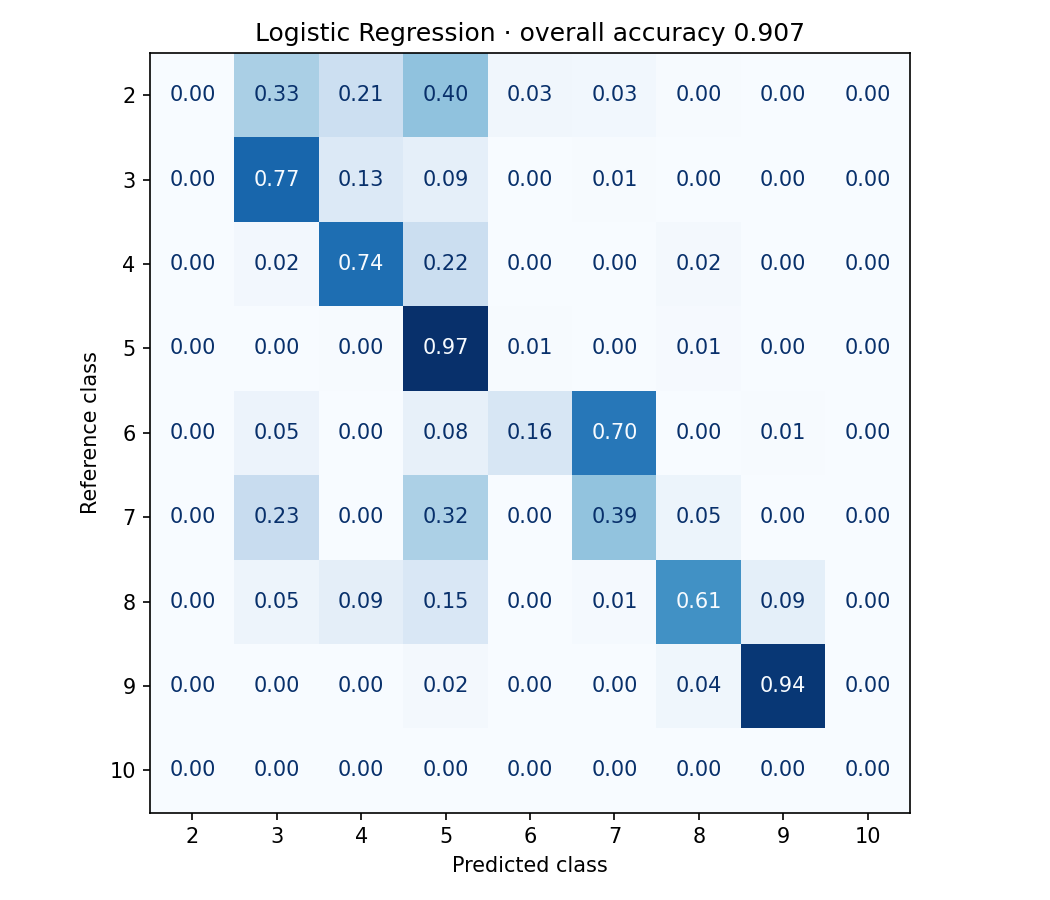
\includegraphics[width=\linewidth]{confusion_matrix_logistic_regression}
\end{subfigure}
\begin{subfigure}{0.49\textwidth}
  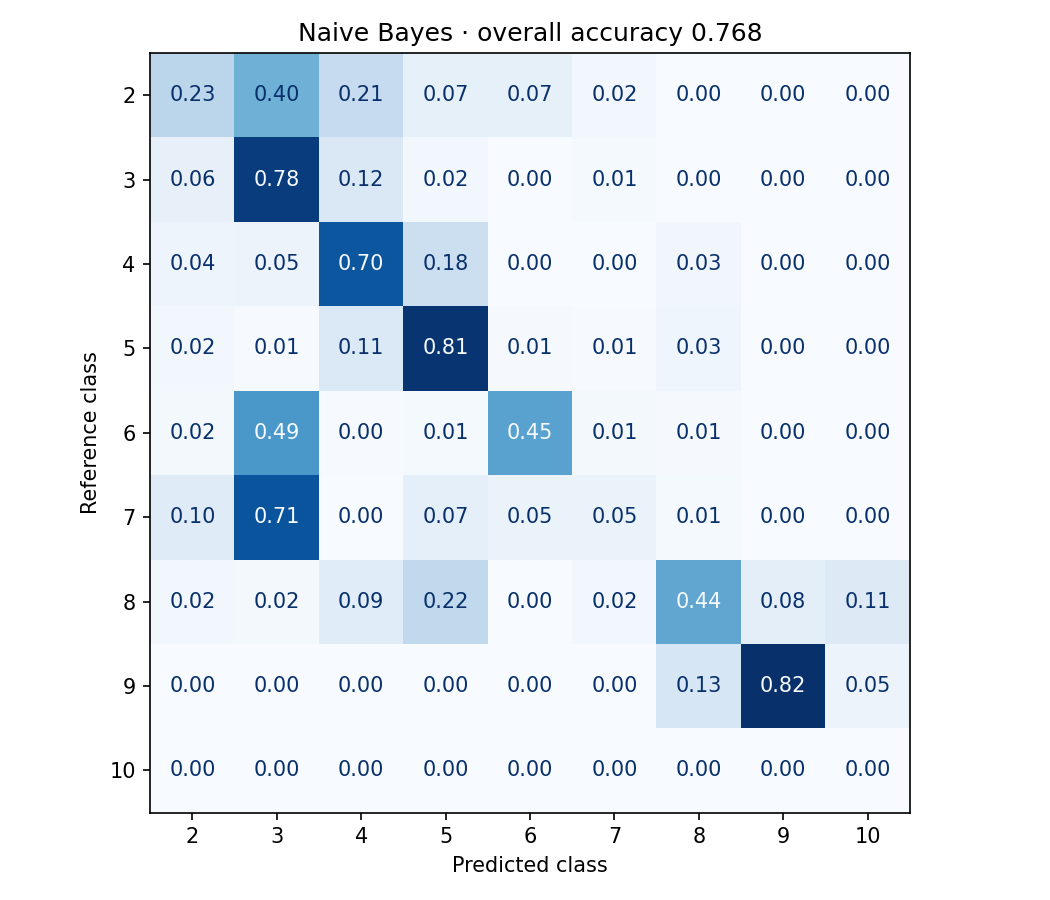
\includegraphics[width=\linewidth]{confusion_matrix_naive_bayes}
\end{subfigure}
\begin{subfigure}{0.49\textwidth}
  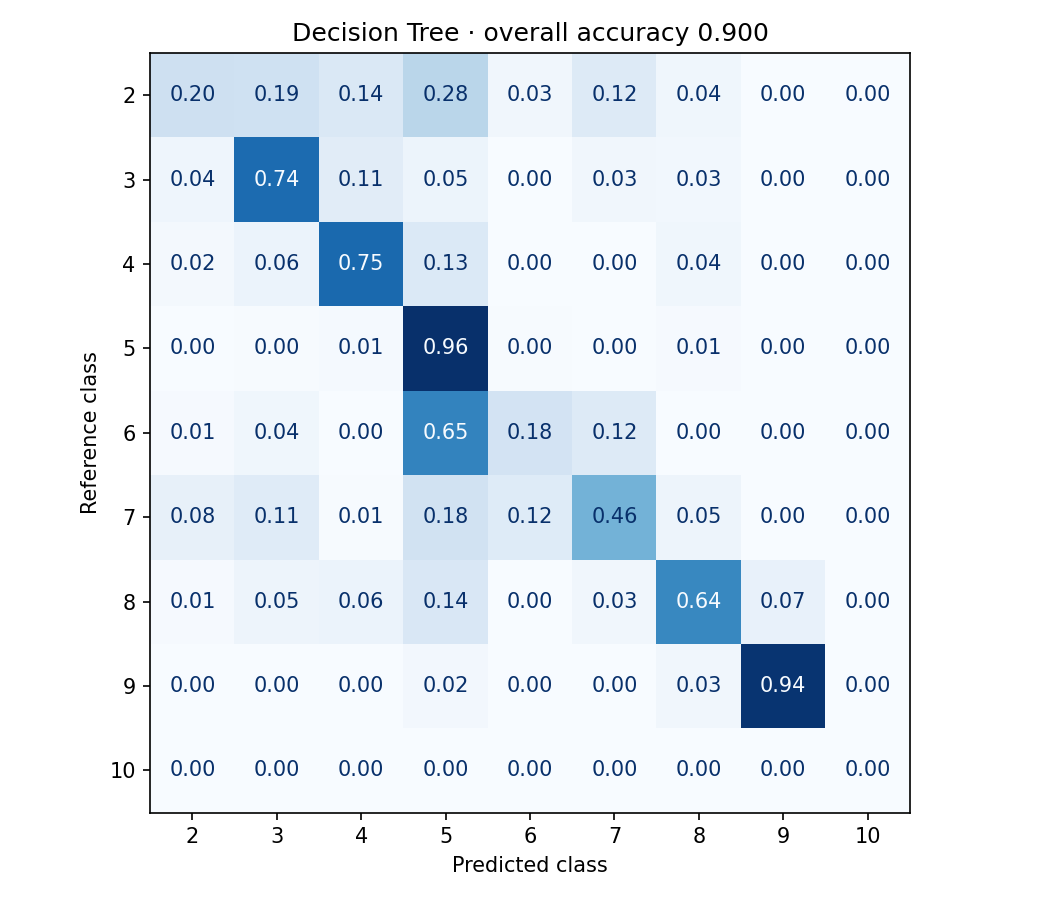
\includegraphics[width=\linewidth]{confusion_matrix_decision_tree}
\end{subfigure}
\caption{Confusion matrices normalised by reference class. The row of class
10 is empty because the class has no test pixels.}
\label{fig:cm}
\end{figure}

\subsection{Recall per class}

Table~\ref{tab:recall} gives the share of each reference class that every
model recovers, which is the diagonal of the normalised matrices.

\begin{table}[H]
\centering\small
\caption{Recall per class on the test set.}
\label{tab:recall}
\begin{tabular}{clrrrr}
\toprule
Class & Land cover & Test pixels & Logistic Regression & Naive Bayes & Decision Tree \\
\midrule
2 & Dark area pixels & 819 & 0.000 & 0.232 & 0.201 \\
3 & Cloud shadows & 6,543 & 0.772 & 0.783 & 0.740 \\
4 & Vegetation & 9,270 & 0.741 & 0.703 & 0.749 \\
5 & Not vegetated & 85,109 & 0.974 & 0.807 & 0.961 \\
6 & Water & 876 & 0.159 & 0.454 & 0.176 \\
7 & Unclassified & 1,302 & 0.395 & 0.055 & 0.459 \\
8 & Cloud medium probability & 4,837 & 0.609 & 0.439 & 0.637 \\
9 & Cloud high probability & 6,090 & 0.944 & 0.823 & 0.945 \\
10 & Thin cirrus & 0 & -- & -- & -- \\
\bottomrule
\end{tabular}

\end{table}

\begin{itemize}
  \item \textbf{Well separated classes.} Not vegetated (5) and cloud high
  probability (9) are recovered above 0.94 by Logistic Regression and the
  Decision Tree. Vegetation (4) and cloud shadows (3) stay around 0.75.
  \item \textbf{Dark area pixels (2).} No model recovers more than a quarter of
  this class, and Logistic Regression assigns none of its 819 test pixels to it;
  they go to not vegetated, cloud shadows and vegetation.
  \item \textbf{Water (6).} Logistic Regression and the Decision Tree recover
  less than 0.18. Logistic Regression sends 70\,\% of the water pixels to class
  7 (unclassified). Naive Bayes does better here (0.45) at the cost of the
  other classes.
  \item \textbf{Cloud medium probability (8)} is confused with not vegetated
  and with cloud high probability, its neighbour in the label scale.
\end{itemize}

\section{Limitations and next steps}

\begin{itemize}
  \item The metrics come from a single train and test split and from default
  hyper-parameters; they are preliminary. Phase 2 will tune each model and
  evaluate it with cross-validation by polygon.
  \item The class imbalance is not corrected. Class weighting or resampling
  will be evaluated for the minority classes, in particular water and dark
  area pixels.
  \item Class 10 cannot be evaluated with one polygon. It will be reported
  separately.
  \item The remaining architectures (K-Nearest Neighbors, Support Vector
  Machines and Artificial Neural Networks) will be added, together with the
  Kappa coefficient, precision, recall and F1-score for the six models.
  \item The best model will classify the full scene to produce the thematic
  raster and the area per class.
\end{itemize}

\appendix
\section{Reproducibility}

The source code lives in the project repository. With the scene archive and
the polygon file under \texttt{data/}, the dataset and the results of this
report are reproduced with these steps:

\begin{enumerate}
  \item Start the stack: \texttt{docker compose up -d}.
  \item Run the Airflow workflows, in this order: \texttt{upload\_bands},
  \texttt{load\_polygons},\\ \texttt{extract\_training\_samples}.
  \item Execute the notebook \texttt{notebooks/01\_phase1\_training.ipynb}.
  \item Generate the tables of this document from the outputs of the notebook:\\
  \texttt{python3 docs/build\_tables.py}.
\end{enumerate}

\end{document}
